\documentclass{article}

\usepackage{graphicx}

\title{Fourier Transform}

\author{Gandhar Vabale EP22B047 (MM22B063)}
\date{16 June, 2023}

\begin{document}
\maketitle

\section*{Fourier Transform in Complex Plane}
Instead of just one formula, I thought it appropriate to also comment a bit on its inverse. The formulae for fourier transform in complex plane are given by

\[
X(j\omega) = \int_{-\infty}^{\infty} x(t) e^{-j\omega t} dt
\]

\[
x(t) = \frac{1}{2\pi} \int_{- \infty } ^ {\infty} X(j\omega) \cdot e^{(j\omega t)} d\omega
\]
\paragraph{}
Here, $j = \sqrt{-1}$, $\omega = 2\pi f$; where f is the frequency of the signal. $x(t)$ is the original function (signal in the context of Electrical department)

\paragraph{}
The equation of $X(j\omega)$ is known as the "Fourier Transform" or "Fourier Integral" of $x(t)$ and the below equation is known as the "Inverse Fourier Transform"

\paragraph{}
These functions are known as the Fourier Transform Pair. The fourier transform converts a given function into a series of frequencies that the original function is composed of.



\paragraph{}
It is used in a variety of applications, like:
\begin{itemize}

\item Modern musical devices
\item Image Compression
\item Image Analysis
\item Image filtering
\item Image reconstruction
\item Machine Learning
\item Signal encoding and decoding

\end{itemize}

\paragraph{}

Since this is a complex function, we cannot simply plot it, but we do not care much about the phase as it is dependent on time translation, here's a plot of fourier coefficients of a signal composed of frequencies 15 and 20.

\begin{center}
	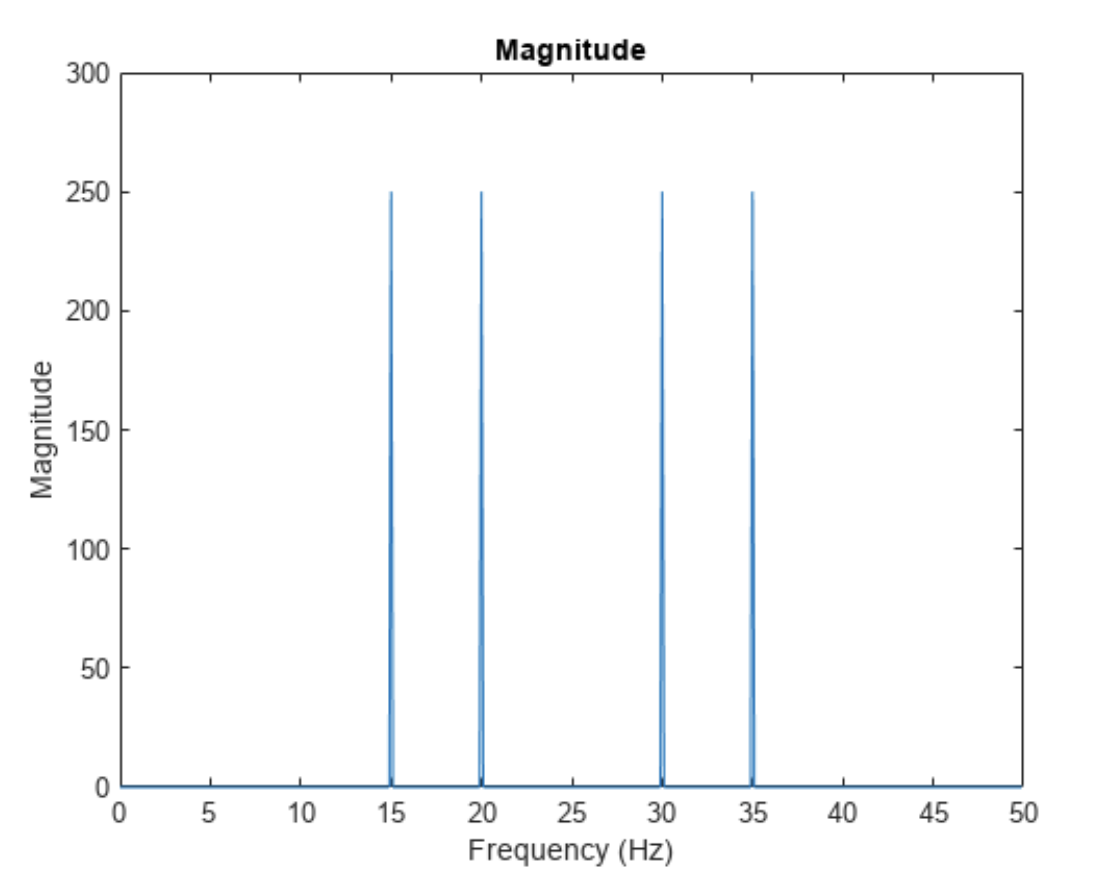
\includegraphics[scale=0.5]{raw.png}
\end{center}

The plot contains four spikes, two for the positive frequencies and two for the negative frequencies. They can be mapped to their original frequencies like this.

\begin{center}
	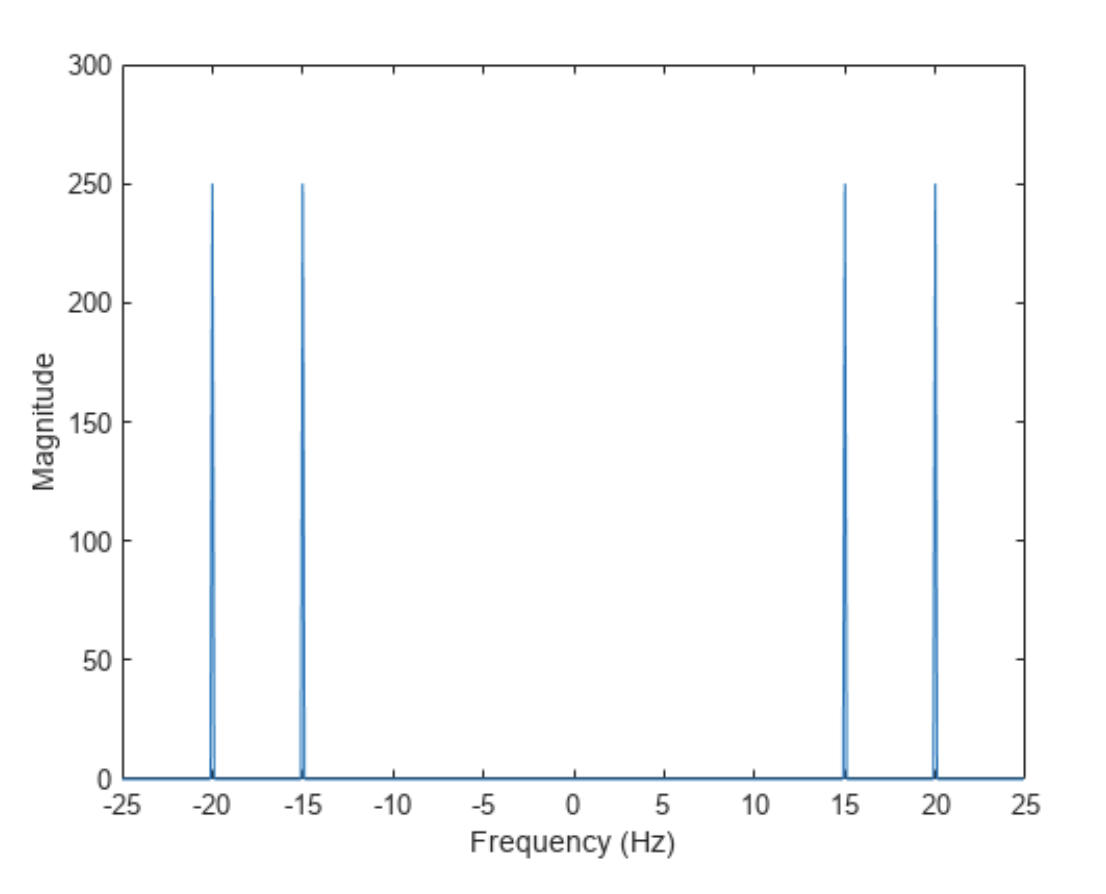
\includegraphics[scale=0.5]{shifted.png}
\end{center}

This function also works in a noisy environment, like daily broadcast channels. With convolution with a high pass and a low pass filter, specific range of frequencies can be specifically be extracted.

\begin{center}
	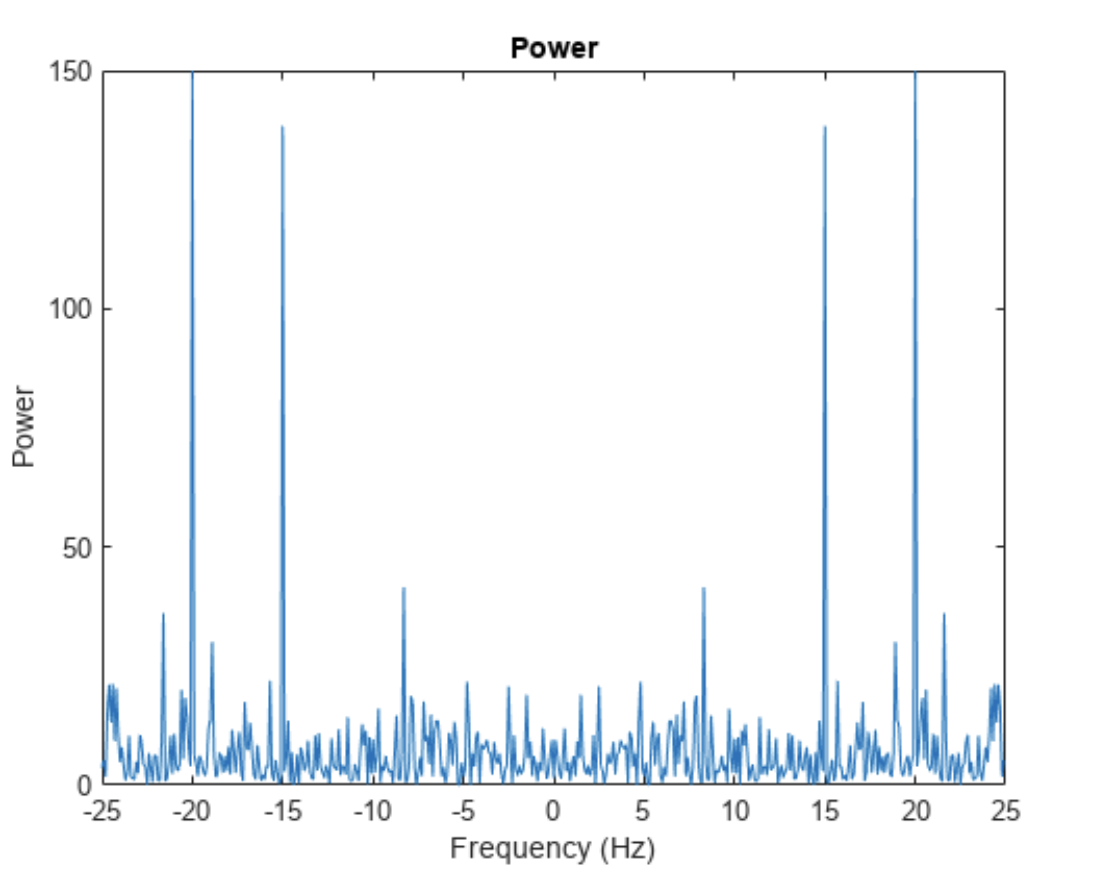
\includegraphics[scale=0.5]{noisy.png}
\end{center}

\paragraph{Choosing the equation}
I first learnt about this equation in the Electrical Department's course "Signals and Systems". We are yet to learnt a lot more about this function, but the number of things I've learnt so far have amazed me. The single best thing I found is the much easier differentiability in complex plane, rather than the conventional use of trigonometric functions, as well as the surprising results of using an exponential.
This property is attributed to all complex exponentials, but in the context of electrical design, give rise to surprising results.
The mere equation $e^{j\pi = -1}$ looks made up. But the fourier transform also solves the problem of not knowing the
fundamental frequency in a function (signal). This is where it becomes extremely helpful in the modern world, as not all functions are periodic.

\paragraph{}
There are a lot of sources to read more about these set of equations and their non-continuous counter parts. But, I'd like to refer to only one book,
Signals and Systems, Second Edition, Alan V. Oppenheim, Alan S. Willsky with Hamid Nawab, but others mentioned in below are good resources too.
The best source though, for me, was from the professor of the course itself, Dr. Anjan Chakravorty, who took a lot of efforts himself to make sure
we learnt, in an extremely compressed time frame, everything that is expected from the course.

\paragraph{}
I do feel that references shouldn't be cited just as footnotes, so I've made them as different section altogether.

\begin{thebibliography}{9}
	\bibitem{textbook}
	Alan V. Oppenheim, Alan S. WillSky with S. Hamid Nawab (1996) \emph{Signals and Systems, Second Edition}, Prentice Hall.

	\bibitem{textbook}
	Robert A. Gabel, Richard A. Roberts \emph{Signals and Linear Systems, Third Edition}, John Wiley \& Sons Canada.
\end{thebibliography}

\end{document}
